\documentclass{article}[18pt]
\usepackage[utf8]{inputenc}
\usepackage[margin=0.7in]{geometry}
\usepackage{parselines} 
\usepackage{amsmath}
\usepackage{titlesec}
\usepackage{pgfplots}
\usepackage{graphicx}
\usepackage[english]{babel}
\usepackage{fancyhdr}
\usepackage{gensymb}
\usepackage{enumerate}
\usepackage{amssymb}
\pgfplotsset{width=10cm,compat=1.9}
\usepackage{tikz}
\usetikzlibrary{calc,shapes.geometric, arrows}
\tikzstyle{startstop} = [rectangle, rounded corners, minimum width=3cm, minimum height=1cm,text centered, draw=black, fill=red!30]
\tikzstyle{io} = [trapezium, trapezium left angle=70, trapezium right angle=110, minimum width=3cm, minimum height=1cm, text centered, draw=black, fill=blue!30]
\tikzstyle{process} = [rectangle, minimum width=3cm, minimum height=1cm, text centered, draw=black, fill=orange!30]
\tikzstyle{decision} = [diamond, minimum width=3cm, minimum height=1cm, text centered, draw=black, fill=green!30,text width=2cm]
\tikzstyle{arrow} = [thick,->,>=stealth]



\titlespacing\section{0pt}{14pt plus 4pt minus 2pt}{0pt plus 2pt minus 2pt}
\newlength\tindent
\setlength{\tindent}{\parindent}
\setlength{\parindent}{0pt}
\renewcommand{\indent}{\hspace*{\tindent}}	
\newcommand{\cred}[1]{\color{red}#1}
\newcommand{\cblue}[1]{\color{blue}#1}
\newcommand{\cgreen}[1]{\color{green}#1}
\hyphenpenalty=10000
\pagestyle{fancy}
\fancyhf{}
\rhead{Sam Robbins 13SE}
\lhead{A Level Maths - D2}
\rfoot{Page \thepage}
\usepackage{float}

\newcommand{\tikzmark}[1]{\tikz[overlay,remember picture] \node (#1) {};}

\newcommand{\DrawVLine}[3][]{%
    \begin{tikzpicture}[overlay,remember picture]
        \draw [#1] ($(#2.north)$) -- ($(#3.north)$);
    \end{tikzpicture}%
}%
\newcommand{\DrawLine}[3][]{%
    \begin{tikzpicture}[overlay,remember picture]
        \draw [#1] ($(#2)+(-0.4,0.6ex)$) -- ($(#3)+(0.6,0.6ex)$);
    \end{tikzpicture}%
}%




\begin{document}
\begin{center}
\underline{\huge Allocation Problems}
\end{center}
\section{Cost Matrices}
\begin{itemize}
\item Require the same number of tasks as workers
\item Only relative costs are important
\end{itemize}
To find a reduced cost matrix:
\begin{enumerate}
\item Subtract the least value in each row from each element of that row
\item Using the new matrix, subtract the least value in each column from each element in that column
\end{enumerate}
\section{Hungarian algorithm}
\begin{enumerate}
\item Find the reduced cost matrix
\item Determine the minimum number of horizontal or vertical straight lines which will cover all the zeros in the matrix
\begin{itemize}
\item If lines $\geqslant$ n, where the matrix is n$\times$n then STOP
\item If lines $<$n, the matrix can be improved and continue 
\end{itemize}
\item Draw in the lines and look for the smallest uncovered element, call it $e$
\item Add $e$ to all covered elements, add it twice if covered twice
\item Subtract $e$ from \textbf{all} elements of the matrix (even those that just had $e$ added)
\item Repeat steps 2-5 until an optimal solution is found
\end{enumerate}
\subsection{Example}
\begin{tabular}{|c|c|c|c|}
\hline
&Dig&Weed&Cut\\
\hline
Boris&250&80&160\\
\hline
Percival&230&90&150\\
\hline
Spike&230&110&140\\
\hline
\end{tabular}\\
\\
\textbf{Find the reduced cost matrix - First process rows}\\
\begin{tabular}{|c|c|c|c|}
\hline
&Dig&Weed&Cut\\
\hline
Boris&170&0&80\\
\hline
Percival&140&0&60\\
\hline
Spike&120&0&30\\
\hline
\end{tabular}\\
\\
\textbf{Find the reduced cost matrix - process columns}\\
\begin{tabular}{|c|c|c|c|}
\hline
&Dig&Weed&Cut\\
\hline
Boris&50&0&50\\
\hline
Percival&20&0&30\\
\hline
Spike&0&0&0\\
\hline
\end{tabular}\\
\textbf{Draw lines to cover zeros}\\
$
\begin{array}{|c|c|c|c|}
\multicolumn{1}{c}{}&
\multicolumn{1}{c}{}&
\multicolumn{1}{c}{\vspace{-.3cm}\tikzmark{StartB}}&
\multicolumn{1}{c}{}\\
\hline
&Dig&Weed&Cut\\
\hline
Boris&50&0&50\\
\hline
Percival&20&0&30\\
\hline
\tikzmark{StartA}Spike&0&0&\tikzmark{EndA}0\\
\hline

\multicolumn{1}{c}{}&
\multicolumn{1}{c}{}&
\multicolumn{1}{c}{\raisebox{.6\normalbaselineskip}{\tikzmark{EndB}}}&
\multicolumn{1}{c}{}\\
\end{array}\\
$
\DrawLine[red, very thick,dotted]{StartA}{EndA}
\DrawVLine[red,very thick,dotted]{StartB}{EndB}
\\
\textbf{Compare to dimension of matrix}\\
2 Lines$\leqslant$3$\times$3 matrix\\
\\
\textbf{Find the smallest uncovered element}\\
20 (Percival digging)\\
\\
\\
\textbf{Add e to all covered elements, and add twice for double covering}\\
\begin{tabular}{|c|c|c|c|}
\hline
&Dig&Weed&Cut\\
\hline
Boris&50&20&50\\
\hline
Percival&20&20&30\\
\hline
Spike&20&40&20\\
\hline
\end{tabular}\\
\\
\textbf{Subtract e from all elements}\\
\begin{tabular}{|c|c|c|c|}
\hline
&Dig&Weed&Cut\\
\hline
Boris&30&0&30\\
\hline
Percival&0&0&10\\
\hline
Spike&0&20&0\\
\hline
\end{tabular}\\
\\
\textbf{Draw lines to cover zeros}\\
\\
$
\begin{array}{|c|c|c|c|}
\multicolumn{1}{c}{}&
\multicolumn{1}{c}{\vspace{-.3cm}\tikzmark{StartA}}&
\multicolumn{1}{c}{\vspace{-.3cm}\tikzmark{StartB}}&
\multicolumn{1}{c}{}\\
\hline
&Dig&Weed&Cut\\
\hline
Boris&30&0&30\\
\hline
Percival&0&0&10\\
\hline
\tikzmark{StartC}Spike&0&20&\tikzmark{EndC}0\\
\hline
\multicolumn{1}{c}{}&
\multicolumn{1}{c}{\raisebox{.6\normalbaselineskip}{\tikzmark{EndA}}}&
\multicolumn{1}{c}{\raisebox{.6\normalbaselineskip}{\tikzmark{EndB}}}&
\multicolumn{1}{c}{}\\
\end{array}\\
$
\DrawVLine[red, very thick,dotted]{StartA}{EndA}
\DrawVLine[red, very thick,dotted]{StartB}{EndB}
\DrawLine[red, very thick,dotted]{StartC}{EndC}
\\
\textbf{Compare to dimension of matrix}\\
3 lines=$3\times3$ matrix - Optimal solution
\section{Dummy Locations}
When the problem is not n$\times$n a dummy location is used, this has zeroes in all the elements.
\subsection{Example}
\begin{tabular}{|c|c|c|c|}
\hline
&Task A&Task B&Task C\\
\hline
Mark&12&23&15\\
\hline
Nicky&14&21&17\\
\hline
Nigel&13&22&20\\
\hline
Susie&14&24&13\\
\hline
\end{tabular}\\
\\
\textbf{Add another task with zero cost}\\
\begin{tabular}{|c|c|c|c|c|}
\hline
&Task A&Task B&Task C&Task D\\
\hline
Mark&12&23&15&0\\
\hline
Nicky&14&21&17&0\\
\hline
Nigel&13&22&20&0\\
\hline
Susie&14&24&13&0\\
\hline
\end{tabular}\\
\\
\textbf{This is then processed as usual}
\section{Incomplete data}
The algorithm can also work on incomplete data (where a person cannot to a task). To do this assign values to the tasks that cannot be done that are at least \textbf{twice as large} as the largest value.
\subsection{Example}
\begin{tabular}{|c|c|c|c|c|}
\hline
&Chinese&French&Indian&Italian\\
\hline
Denis&-&27&15&40\\
\hline
Hilary&14&21&17&13\\
\hline
Robert&20&-&13&-\\
\hline
Trudy&14&24&10&30\\
\hline
\end{tabular}
\newpage
\textbf{The cells with dashes in are then replaced with 100}\\
\begin{tabular}{|c|c|c|c|c|}
\hline
&Chinese&French&Indian&Italian\\
\hline
Denis&\textcolor{red}{100}&27&15&40\\
\hline
Hilary&14&21&17&13\\
\hline
Robert&20&\textcolor{red}{100}&13&\textcolor{red}{100}\\
\hline
Trudy&14&24&10&30\\
\hline
\end{tabular}\\
\\
\textbf{This can then be processed as normal}
\newpage
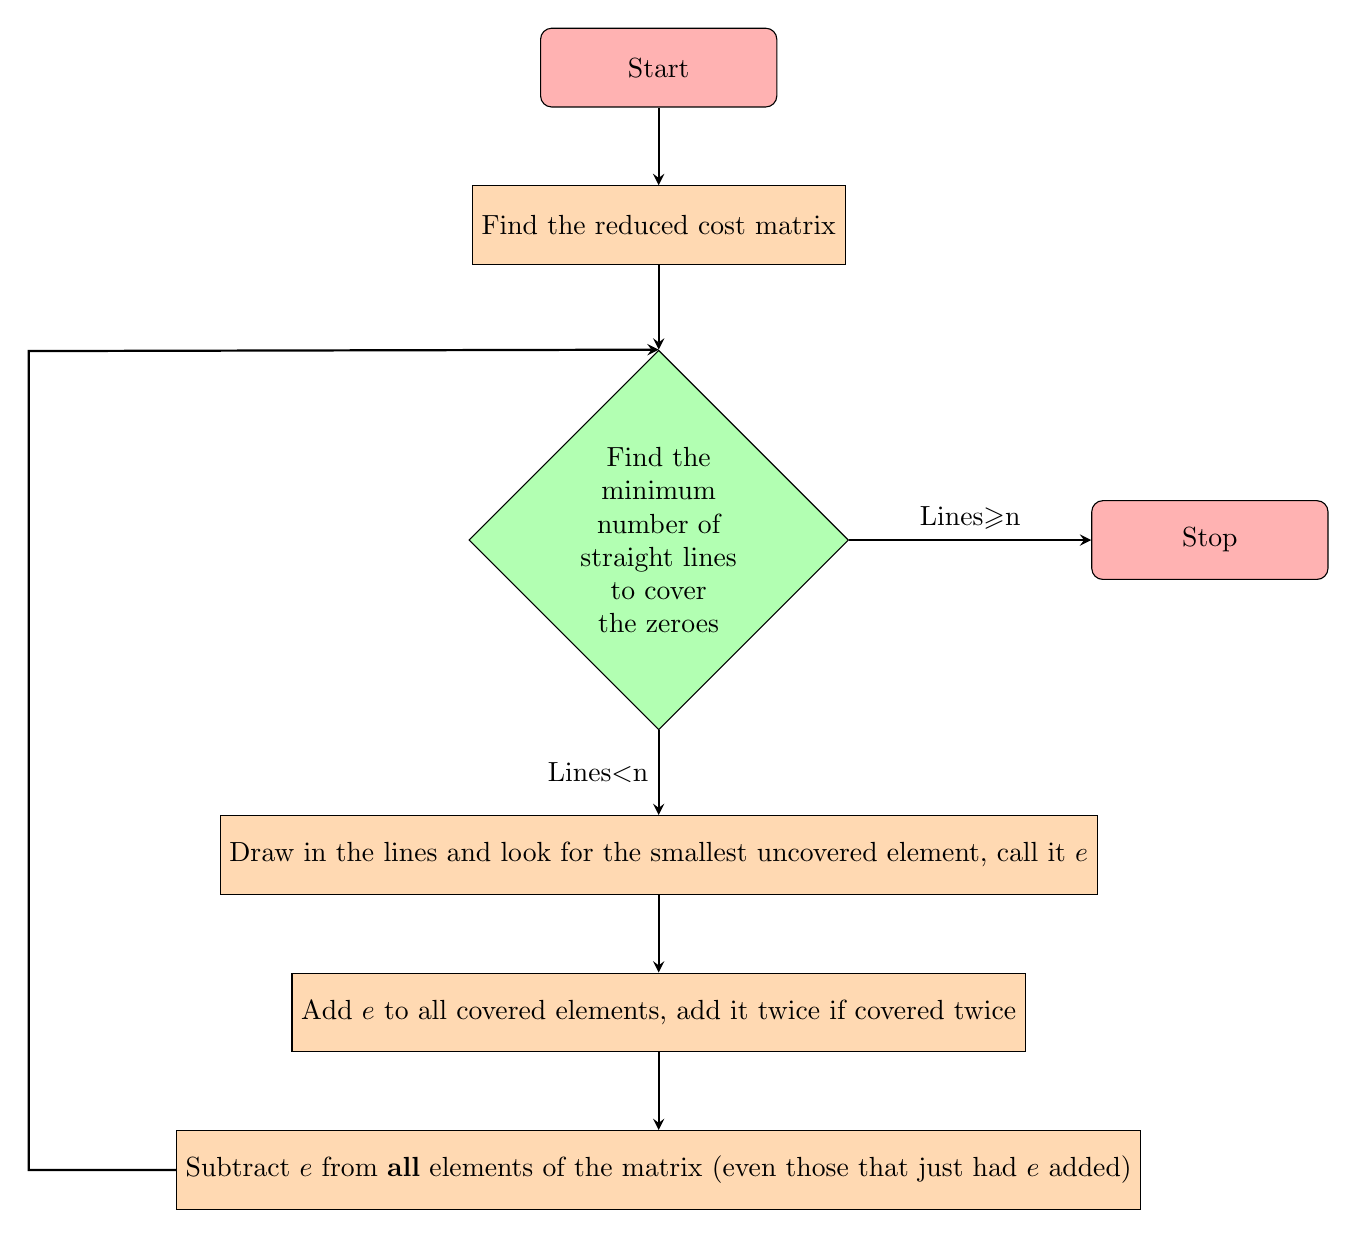
\begin{tikzpicture}[node distance=2cm]
\node (start) [startstop] {Start};
\node (pro1) [process, below of=start] {Find the reduced cost matrix};
\node (dec1) [decision, below of=pro1, yshift=-2cm] {Find the minimum number of straight lines to cover the zeroes};
\node (stop) [startstop, right of=dec1,xshift=5cm] {Stop};
\node (pro2) [process, below of=dec1,yshift=-2cm] {Draw in the lines and look for the smallest uncovered element, call it $e$};
\node (pro3) [process, below of=pro2] {Add $e$ to all covered elements, add it twice if covered twice};
\node (pro4) [process, below of=pro3] {Subtract $e$ from \textbf{all} elements of the matrix (even those that just had $e$ added)};
\draw [arrow] (start) -- (pro1);
\draw [arrow] (pro1) -- (dec1);
\draw [arrow] (dec1) -- node[anchor=east] {Lines$<$n} (pro2);
\draw [arrow] (dec1) -- node[anchor=south] {Lines$\geqslant$n} (stop);
\draw [arrow] (pro2) -- (pro3);
\draw [arrow] (pro3) -- (pro4);
\draw [arrow] (pro4.west) -- (-8,-14) -- (-8,-3.6) -- (dec1.north);




\end{tikzpicture}
\end{document}
